\documentclass[conference,onecolumn]{IEEEtran}
\usepackage[T1]{fontenc}
\usepackage{amsmath,amssymb,booktabs,graphicx}
\usepackage[hidelinks]{hyperref}
\hypersetup{
  pdftitle={A Parallel Two-Dimensional FFT with MPI},
  pdfauthor={Samuele Mega},
  pdfsubject={Strong-scaling analysis of a distributed two-dimensional FFT}
}
% Plain caption style instead of IEEEtran's centered small caps.
\usepackage{caption}
\captionsetup{font=footnotesize,labelfont=bf,labelsep=period}
\captionsetup[table]{position=above}
\renewcommand{\thetable}{\arabic{table}}
\renewcommand{\tablename}{Table}
\renewcommand{\figurename}{Figure}
% IEEEtran centers small-caps section titles for its two-column layout; in
% one column they look lost, so sections use left-aligned bold headings.
\makeatletter
\renewcommand{\section}{\@startsection{section}{1}{\z@}%
  {2.6ex plus 1ex minus .2ex}{1.2ex plus .2ex}%
  {\normalfont\large\bfseries}}
\renewcommand{\subsection}{\@startsection{subsection}{2}{\z@}%
  {2.2ex plus .8ex minus .2ex}{1ex plus .2ex}%
  {\normalfont\normalsize\bfseries}}
\makeatother
\renewcommand{\thesection}{\arabic{section}}
\renewcommand{\thesectiondis}{\arabic{section}.}
\renewcommand{\thesubsection}{\thesection.\arabic{subsection}}
\renewcommand{\thesubsectiondis}{\thesubsection}
% Pack float-only pages from the top instead of stretching the gaps.
\makeatletter
\setlength{\@fptop}{0pt}
\setlength{\@fpsep}{8pt plus 1fil}
\makeatother
\raggedbottom
% Definition, proposition and proof set apart from the running text:
% bold heading, italic body, vertical space around, and QED to close.
\usepackage{amsthm}
\newtheoremstyle{course}%
  {1.6ex plus .5ex minus .2ex}{1.6ex plus .5ex minus .2ex}%
  {\itshape}{}{\bfseries}{.}{ }%
  {\thmname{#1}\thmnumber{ #2}\thmnote{ (#3)}}
\theoremstyle{course}
\newtheorem{definition}{Definition}
\newtheorem{proposition}{Proposition}
\renewcommand{\qedsymbol}{QED}
\renewenvironment{proof}{\par\addvspace{.8ex plus .3ex}%
  \noindent\textbf{Proof.}\ \ignorespaces}%
  {\qed\par\addvspace{1.6ex plus .5ex minus .2ex}}
\newif\ifFinalCampaign
\FinalCampaignfalse
\title{A Parallel Two-Dimensional FFT with MPI}
\author{\IEEEauthorblockN{Samuele Mega}
\IEEEauthorblockA{Parallel Computing Laboratory, University of Padova}}
\begin{document}
\maketitle
\begin{abstract}
This report describes the design, the implementation, and the measurement
of a parallel algorithm for the two-dimensional discrete Fourier transform,
written in C with MPI. Two programs have been developed, a sequential one
and a parallel one, both built on the same radix-2 kernel. In the parallel
program, each process owns a slab of complete rows of the matrix, so that
every butterfly is executed locally and communication is confined to a
distributed transpose, performed twice: once to change the axis being
transformed and once to restore the original layout. The number of
processes is restricted to a power of two, so that the exchange can be read
on the binary hypercube studied in the course, in addition to the complete
graph. The strong scaling of the forward transform has been measured on the
CAPRI system for three matrices with the same number of elements, one
square, one wide, and one tall. The three behave almost identically, with
parallel efficiency of approximately $75\%$ up to 16 processes; beyond this
point the speedup saturates near 14. The ceiling does not move when the number of
elements is quadrupled, hence the startup cost of the collective exchange
cannot, by itself, explain it.
\end{abstract}

\section{Introduction}
Two-dimensional Fourier transforms dominate the time step of spectral
solvers for periodic fluid problems, where the field is transformed at every
step to evaluate its derivatives in the frequency domain, and transformed
back afterwards. The idea of the project originated in that context. Here,
however, we study the transform by itself, without a fluid solver on top of
it: the object of this report is the transform, its parallelization with
MPI, and the measurement of the resulting performance on CAPRI.

\subsection{Problem Formulation}
We begin by defining the computational problem, in the notation
of~\cite[ch.~6]{alg}.

\begin{definition}[Two-dimensional DFT]
Let $A$ be an $N_y\times N_x$ complex matrix and let $\omega_n=e^{-2\pi i/n}$
denote an $n$-th principal root of unity. The forward two-dimensional
discrete Fourier transform of $A$ is the $N_y\times N_x$ matrix $X$ with
entries
\begin{equation}
 X_{k_y,k_x}=\sum_{y=0}^{N_y-1}\sum_{x=0}^{N_x-1} A_{y,x}\,
 \omega_{N_y}^{k_y y}\,\omega_{N_x}^{k_x x},
 \qquad 0\le k_y<N_y,\quad 0\le k_x<N_x. \label{eq:dft2}
\end{equation}
\end{definition}

The inverse transform is obtained by replacing the roots with their
conjugates and dividing the result by $N_yN_x$. Throughout the report, both
dimensions are assumed to be powers of two. They need not be equal, and
either may equal one, in which case the transform degenerates to a
one-dimensional one. We let $N=N_yN_x$ denote the number of elements of the
matrix.

\subsection{Objectives}
The transform has been implemented twice, in a sequential program and in an
MPI program, both written in C and both built on the same one-dimensional
kernel. Every invocation of either program measures one forward transform
of an $N_y\times N_x$ pseudo-random matrix, generated from a seed as
described in Section~\ref{sec:method}, and reports the measured time
together with the fraction of that time spent in local arithmetic. The
project has been carried out individually, following the timeline of the
laboratory~\cite{lab}: sequential algorithm first, then design and MPI
implementation of the parallel one, then measurements on CAPRI.

The performance question we are interested in is one of strong scaling,
that is, how the time of the transform changes with the number $P$ of
processes when the matrix is kept fixed. Three matrices with the same number
of elements are measured separately: a square one, a wide one with half the
rows and twice the columns, and the tall transpose of the wide one. Since,
as we shall see, the arithmetic work depends on the dimensions only through
their product, the comparison isolates the effect of the shape on the rest
of the computation.

\section{The Sequential Algorithm}\label{sec:seq}

\subsection{Separability}\label{sec:sep}
The exponential in Equation~\ref{eq:dft2} is the product of a factor that
depends only on $(y,k_y)$ and of a factor that depends only on $(x,k_x)$,
so the double sum can be evaluated one axis at a time:
\[
 X_{k_y,k_x}=\sum_{y=0}^{N_y-1}\omega_{N_y}^{k_y y}
 \Bigl(\sum_{x=0}^{N_x-1}A_{y,x}\,\omega_{N_x}^{k_x x}\Bigr).
\]
The inner sum is the one-dimensional DFT of row $y$ of $A$; the outer sum
is the one-dimensional DFT of column $k_x$ of the matrix of row transforms.
The two-dimensional transform is therefore \emph{separable}: it is computed
by transforming all the $N_y$ rows with a DFT of order $N_x$, and then all
the $N_x$ columns of the result with a DFT of order $N_y$. Nothing needs to
be done between the two phases.

\subsection{The Radix-2 Kernel}
Both programs use the same one-dimensional kernel: the iterative,
decimation-in-frequency FFT of~\cite[sec.~6.3]{alg}, that is, the
factorization $(2,n/2)$ applied at every level of the recursion for a
transform of order $n=2^m$. The recursion unfolds into $\log_2 n$ stages. A
stage of width $w$, for $w=n,n/2,\ldots,2$, applies the butterfly
\begin{equation}
 (a,b)\;\longmapsto\;\bigl(a+b,\;(a-b)\,\omega_w^{j}\bigr),
 \qquad 0\le j<w/2, \label{eq:butterfly}
\end{equation}
to every pair $(a,b)$ of elements at distance $w/2$ within each block of $w$
consecutive positions. After the last stage the components of the transform
appear in bit-reversed order, and a final permutation restores the natural
order. The kernel is unnormalized in both directions; the two-dimensional
inverse divides by $N_yN_x$ once, at the end.

We measure the arithmetic in butterflies, each consisting of one complex
multiplication and two complex additions.

\begin{proposition}[Work of the two-dimensional transform]\label{prop:work}
The transform of an $N_y\times N_x$ matrix, computed by rows and then by
columns as in Section~\ref{sec:sep}, executes
\begin{equation}
 B=\frac{N_yN_x}{2}\bigl(\log_2 N_x+\log_2 N_y\bigr)=\frac{N}{2}\log_2 N
 \label{eq:work}
\end{equation}
butterflies, hence its work is $\theta(N\log N)$.
\end{proposition}

\begin{proof}
A transform of order $n$ executes $\log_2 n$ stages of $n/2$ butterflies
each, for a total of $(n/2)\log_2 n$. The row phase executes $N_y$
transforms of order $N_x$ and the column phase $N_x$ transforms of order
$N_y$. Adding the two contributions and using
$\log_2 N_x+\log_2 N_y=\log_2(N_xN_y)$ yields Equation~\ref{eq:work}.
\end{proof}

Since $B$ depends on the dimensions only through their product $N$, two
matrices with the same number of elements, however different in shape,
require exactly the same number of butterflies. We will use this fact when
comparing the three matrices of the experiments.

\subsection{Organization of the Program}
The program keeps the matrix and one scratch buffer of the same size, and
proceeds in four steps.
\begin{enumerate}
\itemsep1pt
\item The $N_y$ rows are transformed in place, which costs
$(N/2)\log_2 N_x$ butterflies.
\item The matrix is transposed into the scratch buffer, moving $N$
elements.
\item The $N_x$ rows of the transposed matrix, which are the columns of the
original one, are transformed in place, which costs $(N/2)\log_2 N_y$
butterflies.
\item The matrix is transposed back into the original buffer, moving $N$
elements again.
\end{enumerate}
The two transposes cost $\theta(N)$ memory traffic and no floating-point
work; their purpose is to let the kernel always operate on contiguous rows,
and to return the result in the row-major layout of the input.

\section{The Parallel Algorithm}\label{sec:par}

\subsection{Data Distribution}
With $P$ processes, numbered $0,1,\ldots,P-1$, process $r$ holds the
$N_y/P$ consecutive rows of $A$ with indices $rN_y/P,\ldots,(r+1)N_y/P-1$,
which we call its \emph{row slab}, and is responsible for the same rows of
the output $X$. We require that $P=2^d$ be a power of two and that
$P\le\min(N_y,N_x)$, so that both the rows and the columns of the matrix
divide evenly among the processes. The restriction to powers of two is not
needed by the algorithm itself; it is imposed to give the algorithm a
reading on the hypercube, as discussed in Section~\ref{sec:topology}.

\subsection{The Algorithm}
The steps mirror those of the sequential program, with the local transposes
replaced by a redistribution of the matrix among the processes.
\begin{enumerate}
\itemsep1pt
\item Each process transforms its $N_y/P$ rows, with no communication,
executing $(N/2P)\log_2 N_x$ butterflies.
\item A \emph{distributed transpose} redistributes the matrix, so that
process $r$ holds the $N_x/P$ complete rows of the transposed matrix with
indices $rN_x/P,\ldots,(r+1)N_x/P-1$. This is the first communication
step.
\item Each process transforms its new rows, that is, the original columns,
executing $(N/2P)\log_2 N_y$ butterflies.
\item A second distributed transpose, the second and last communication
step, restores the row slabs of the original layout.
\end{enumerate}
Every butterfly is executed locally, and the work per process is exactly
$B/P$: the arithmetic is perfectly balanced. All the communication is
concentrated in the two transposes.

It is easy to see what each transpose moves. The elements that process $r$
must send to process $s$ are those in the rows of $r$ and in the columns of
$s$, which form a block of $(N_y/P)\times(N_x/P)=N/P^2$ elements. Every
pair of distinct processes therefore exchanges exactly one such block, and
each process sends and receives $(P-1)N/P^2<N/P$ elements in total. This
pattern is an \emph{all-to-all} exchange with blocks of equal size, and it
is implemented as such: the sender packs, for each destination, the columns
of its slab belonging to that destination into a contiguous block; a single
call to \texttt{MPI\_Alltoall}~\cite{mpi} exchanges the $P$ blocks; the
receiver unpacks each block, writing its elements at transposed indices. A
process keeps four buffers of $N/P$ elements each: the slab, the transposed
slab, the send buffer, and the receive buffer. Each process also generates
its own rows of the input directly, as explained in Section~\ref{sec:method},
so that no process ever stores the whole matrix.

\subsection{Parallelism Left Unused}
The decomposition leaves further parallelism unused: a process transforms
its $N_y/P$ rows one after the other, and within one transform the $n/2$
butterflies of a stage are independent. This is deliberate. The row level
alone admits $P\le\min(N_y,N_x)$ processes, that is, up to 8192 even for
the least favorable of the three matrices measured here, against the 256
cores of the machine; at the largest process count measured, each process
still holds hundreds of complete rows. A finer decomposition is therefore
not needed to expose enough concurrency to occupy all the available cores,
although it might have other advantages, which we do not explore here.
Splitting a single one-dimensional transform across processes is the
alternative organization discussed in Section~\ref{sec:topology}, which
moves communication inside the computation rather than reducing it, and
threading inside a process would turn the program into a hybrid MPI+OpenMP
one, outside the scope of the project.

\section{Topology and Communication Cost}\label{sec:topology}
MPI does not restrict which pairs of processes may exchange messages: any
process can send to any other. The complete graph $K_P$
of~\cite[sec.~1.1]{arch} is therefore the natural \emph{logical} model of
the communication that MPI offers to the program. The physical network
underneath may have any topology; the model makes no claim about it.

\subsection{The Complete Graph}
On $K_P$, the distributed transpose runs as $P-1$ direct block transfers
per process, each of $N/P^2$ elements, over the edges $(r,s)$, which in
$K_P$ always exist. There is no forwarding: every element traverses exactly
one edge. In the multi-port processor-network model of~\cite[sec.~1]{arch},
the $P-1$ transfers of a node could even proceed simultaneously, one per
port. The cost model of Section~\ref{sec:cost} will be less generous, in
order to reflect how an MPI library actually sends messages.

\subsection{The Hypercube}\label{sec:hcube}
The restriction $P=2^d$ gives the algorithm a second reading, on the binary
hypercube $H_d$ of~\cite[ch.~3]{arch}. As for the complete graph, this is
an algorithmic interpretation, not a description of the machine.

We recall from~\cite[sec.~3.3]{arch} why the FFT and the hypercube are
related. In the decimation-in-frequency FFT of order $n=2^m$, the stage of
width $2^{j+1}$ pairs each index with the index that differs from it only
in bit $j$. If line $i$ of the CDAG is assigned to node $i$ of $H_m$, these
pairs are exactly the edges of dimension $j$ of the hypercube, and the
stages activate the dimensions in the order $m-1,m-2,\ldots,0$: the FFT is
a DESCEND algorithm. When the order $n$ exceeds the number $P=2^d$ of
nodes, each node holds $n/P$ consecutive elements, the first $d$ stages
require one communication along one dimension each, and the remaining
stages are local. This organization, known as \emph{binary exchange}, could
be applied to each row and column transform of Section~\ref{sec:sep}.

The implementation follows a different organization, which we call the
\emph{transpose algorithm}: the rows are kept whole, so that every stage of
every transform is local, and the communication is confined to the two
distributed transposes. In this organization the hypercube describes the
exchange rather than the butterflies. The exchange can be carried out on
$H_d$ in $d$ steps, one per dimension: in step $j$, each node keeps the
elements whose destination agrees with its own index in bit $j$, and sends
the others, which are half of what it holds, to its neighbour across
dimension $j$. After the $d$ steps every element has reached its
destination, having traversed one edge for each bit in which source and
destination differ, exactly as in the shortest paths of the hypercube. Each
node moves $N/2P$ elements per step, hence $(N/2P)\log_2 P$ in total:
fewer transfers than on the complete graph, $\log_2 P$ instead of $P-1$,
but a larger volume, which is the price of forwarding.

\subsection{A Simple Cost Model}\label{sec:cost}
Let the cost of a message of $m$ elements be $t_s+m\,t_w$, where $t_s$ is a
fixed startup time and $t_w$ the transfer time per element. For $K_P$, we
adopt a pairwise-exchange model in which the $P-1$ blocks sent by each
process are separate messages, each contributing its own startup cost. This
is an implementation-oriented model of \texttt{MPI\_Alltoall}, rather than
the multi-port processor-network cost of $K_P$ itself. For $H_d$, we charge
one message per step of the exchange of Section~\ref{sec:hcube}. One
transpose then costs
\begin{align}
 T_{K_P}&=(P-1)\left(t_s+\frac{N}{P^2}\,t_w\right) \label{eq:tkp}\\
 T_{H_d}&=\log_2 P\left(t_s+\frac{N}{2P}\,t_w\right) \label{eq:thd}
\end{align}
on the complete graph and on the hypercube, respectively. For small $P$ the
startup term of Equation~\ref{eq:tkp} is negligible and the complete graph
wins; for large $P$ the term $P\,t_s$ grows and the hypercube wins. An MPI
library may implement \texttt{MPI\_Alltoall} in either way, or in others;
the program leaves the choice to the library.

Let $t_c$ be the time per butterfly. Combining Proposition~\ref{prop:work}
with Equation~\ref{eq:tkp}, a rough model of the parallel time is
\begin{equation}
 T_P\approx\frac{N\log_2 N}{2P}\,t_c
 +2\left(P\,t_s+\frac{N}{P}\,t_w\right)+c_{\mathrm{mem}}\frac{N}{P},
 \label{eq:model}
\end{equation}
where the last term accounts for packing, unpacking, and local memory
traffic. The model is idealized, but it supports two qualitative
predictions. First, the arithmetic term and the transfer term both scale as
$1/P$, while the startup term grows with $P$; efficiency must therefore
drop once $N/P$ becomes small. Second, if the startup term were the binding
one, equating it with the arithmetic term would place the saturation point
at
\begin{equation}
 P^\star\propto\sqrt{N\log_2 N}, \label{eq:pstar}
\end{equation}
so that a matrix with four times as many elements should move the knee of
the speedup curve by about a factor of two toward larger $P$.
Equation~\ref{eq:pstar} follows from the pairwise model, whose startup term
grows as $P\,t_s$; it is a property of that model, not of the FFT or of the
complete graph. The second prediction can be checked against the
measurements, and we will do so in Section~\ref{sec:concl}.

\section{Correctness}\label{sec:correct}
Both programs have been checked against a direct $O(N^2)$ evaluation of
Equation~\ref{eq:dft2}, with acceptance criterion
\[
 \frac{\lVert x-r\rVert_2}{\max(\lVert r\rVert_2,1)}\le 10^{-10},
\]
where $x$ is the computed transform and $r$ the reference. The tests cover
forward transforms, inverse round trips, square matrices, both rectangular
orientations, and the degenerate shapes with a dimension equal to one; for
the MPI program, the same comparisons at $P=1,2,4$ after gathering the
slabs; and the rejection of invalid dimensions, seeds, and process counts.
The largest error observed across these checks was about
$7\times10^{-15}$. A further check verifies that generating a slab at an
offset reproduces the corresponding part of the full matrix; this is the
property that allows each process to generate its own rows.

\section{Measurement Method}\label{sec:method}

\subsection{The Input}
The input matrix is deterministic. Element $k$ of the matrix, in row-major
order, is obtained from a 64-bit pseudo-random generator whose state before
element $k$ depends only on the seed and on $k$; its real and imaginary
components lie in $[-0.5,0.5)$. Hence the same dimensions and seed
reproduce the same matrix on any machine, without input files, and a
process can generate its slab without generating what precedes it.

\subsection{Timers and Metrics}
Every invocation measures one forward transform. Allocation and input
generation take place first, outside the timed region. The timed kernel
covers the two FFT phases, the computation of the twiddle factors, and both
transposes, including packing and unpacking in the MPI program. The twiddle
factors are computed inside the kernel by evaluating the complex
exponential at every stage; the time per butterfly $t_c$ of
Section~\ref{sec:cost} is therefore an effective average cost, which
includes a share of that evaluation, rather than the cost of the arithmetic
operations alone. The processes synchronize with a barrier right before the kernel; each process
$r$ measures its own kernel time $T_r$, and the reported time is
$T_P=\max_r T_r$. Two auxiliary timers measure the local FFT phases alone,
giving a time $F_r$ per process. We define the compute fraction $f$, the
speedup $S(P)$, and the parallel efficiency $E(P)$~\cite{lab} as
\begin{equation}
 f=\frac{\sum_r F_r}{\sum_r T_r},\qquad
 S(P)=\frac{\operatorname{median}(T_{\mathrm{seq}})}{\operatorname{median}(T_P)},\qquad
 E(P)=\frac{S(P)}{P}. \label{eq:metrics}
\end{equation}
where $T_{\mathrm{seq}}$ is the time of the sequential program. The
complement of $f$ contains packing, unpacking, communication, and waiting, so $1-f$ cannot be
read as pure network time. Every measured
point is repeated in twenty independent invocations; the tables report the
medians, and the spread between minimum and maximum is stated with the
results.

\subsection{Experimental Setup}
All measurements ran on CAPRI, a single HPE Superdome Flex system: 16 Intel
Xeon Gold 6130 processors of 16 cores each, 256 cores in total, in four
interconnected chassis, with 6~TB of shared memory, presented to Slurm as
one node~\cite{capri}. All processes therefore run within one shared-memory
system, and no multi-node network is involved, although the processes may
be placed on different sockets and chassis. The programs were compiled with
gcc~7.5.0 (\texttt{-O3 -std=c11}) against Open~MPI~2.1.6.

Each campaign was submitted with \texttt{sbatch} as a single job on the
\texttt{allgroups} partition, with as many tasks as the largest $P$ of the
campaign: 16 for the 8192-base matrices, 32 for the 16384-base ones, and 64
for the exploratory campaign of Section~\ref{sec:concl}. The job ran, for
each shape, each $P$, and each repetition,
\begin{center}
\texttt{mpirun -np P ./fft2d\_mpi NY NX 42 RUN}
\end{center}
and \texttt{./fft2d\_seq NY NX 42 RUN} for the sequential baseline, where
42 is the seed used throughout and \texttt{RUN} the repetition index. Each
MPI rank is a single-threaded process. No explicit core binding was
requested, in line with the laboratory material, which does not require it;
this is an experimental limitation, since the placement of the processes on
the cores, and hence across sockets and chassis, is left to the system. The
machine was shared with other workloads during the measurements.

\section{Results}\label{sec:results}
\IfFileExists{generated/results.tex}{%
\input{generated/results.tex}
\begin{table}[!t]
\caption{Median kernel measurements for the three matrices. For each
matrix and each number of processes $P$, the columns report the median
kernel time $t$, the compute fraction $f$, and the speedup $S$ of
Equation~\ref{eq:metrics}. The first row is the sequential program. Lower is
better for $t$; higher is better for $f$ and $S$.}
\label{tab:kernel}
\centering\small
\input{generated/table-kernel.tex}
\end{table}
\begin{figure}[!t]
\centering

\includegraphics[width=\columnwidth]{generated/overview.pdf}
\caption{Strong scaling of the three matrices. The left panel shows the
median speedup $S(P)$ against the number of processes, with the ideal
$S(P)=P$ as a reference; the right panel shows the compute fraction $f$.
The three curves are nearly superimposed, as Proposition~\ref{prop:work}
leads one to expect. Higher is better in both panels.}
\label{fig:overview}
\end{figure}
}{
No measurements have been supplied to this report build; run a benchmark
campaign and rebuild the report on its results directory.
}

\section{Conclusions}\label{sec:concl}
Let us first summarize what the design guarantees. The sequential and the
MPI programs share the same kernel, so the speedups compare equal
arithmetic. Keeping the rows whole moves all the communication into two
collective exchanges, and returning the result in the original layout costs
the second one. The three matrices perform almost identically at equal
element count, as Proposition~\ref{prop:work} predicts: the butterfly count
depends on the dimensions only through $\log_2 N_x+\log_2 N_y=\log_2 N$.

Strong scaling is good through $P=16$, where the parallel efficiency is
still approximately $75\%$. Beyond that point the non-compute overhead grows
quickly, the compute fraction falls to about one third at $P=32$, and the
speedup settles near $13.9$. As for scalability, therefore, $S(P)$ does not
always increase: the measured implementation ceases to obtain significant
speedup beyond $P\approx16$--$32$. It ought to be kept in mind that this is
a property of this transpose-based MPI implementation on this machine, not
an exhaustion of the parallelism of the FFT, which Section~\ref{sec:par}
shows to be far larger. The design has two further weaknesses. At $P=1$ the
MPI program
is about $6\%$ slower than the sequential one, because it still packs,
unpacks, and calls the collective with a single participant. Moreover, the
compute fraction is only $0.68$ already in the sequential program: the two
local transposes and the memory traffic they cause are a sizable share of
the kernel even before any communication takes place.

\subsection{An Exploratory Campaign on Larger Matrices}
According to Equation~\ref{eq:pstar}, the ceiling should move with the size
of the problem, if the startup term is the binding one. An exploratory
campaign on matrices with four times as many elements reproduces the same
ceiling and extends the curve to $P=64$ (Table~\ref{tab:extra}).
Figure~\ref{fig:sizes} compares the square-matrix curves at three sizes: an
equivalent twenty-run campaign on 8192-base matrices, the 16384 campaign of
Section~\ref{sec:results}, and the exploratory 32768 one.
\begin{table}[t]
\caption{Exploratory campaign: square $32768\times32768$ matrix
($16$~GiB of data; the full program footprint is 32~GiB sequentially and
64~GiB for MPI), five repetitions per point. The wide and tall shapes
showed the same behavior (data omitted). Lower is better for the time; higher
is better for $f$ and $S(P)$.}
\label{tab:extra}
\centering\small
\begin{tabular}{lrrrr}\toprule
Version & $P$ & Median time (s) & $f$ & $S(P)$\\\midrule
seq & 1 & 295.8 & 0.702 & 1.000\\
mpi & 1 & 316.2 & 0.660 & 0.936\\
mpi & 2 & 155.8 & 0.668 & 1.899\\
mpi & 4 & 84.3 & 0.617 & 3.510\\
mpi & 8 & 43.2 & 0.602 & 6.847\\
mpi & 16 & 22.0 & 0.596 & 13.467\\
mpi & 32 & 21.5 & 0.357 & 13.773\\
mpi & 64 & 22.3 & 0.243 & 13.243\\
\bottomrule\end{tabular}
\end{table}
\begin{figure}[t]
\centering
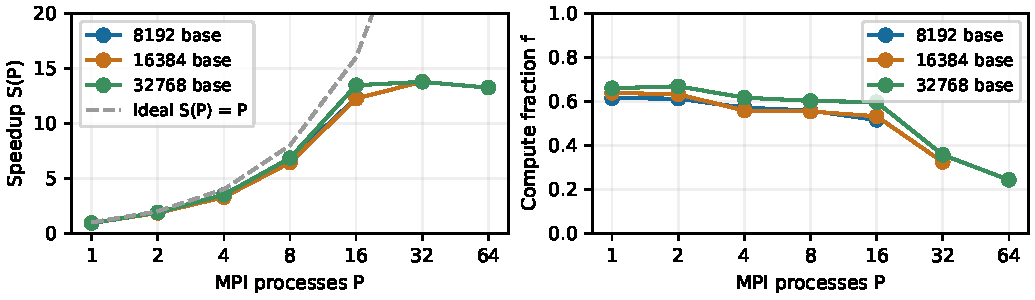
\includegraphics[width=\columnwidth]{../results/scaling-sizes.pdf}
\caption{Square-matrix speedup (left) and compute fraction (right) across
sizes; twenty repetitions per point for 8192 and 16384, five for 32768.
Higher is better in both panels. If the startup term were binding, the knee
of the curves should shift to the right by about a factor of two at each
step in size.}
\label{fig:sizes}
\end{figure}

\subsection{Interpreting the Ceiling}
The ceiling is the main experimental result.
\begin{enumerate}
\item The 32768 matrices contain four times as many elements as the 16384
ones and require about $4.3$ times the FFT arithmetic, yet the maximum
speedup stays at about $13$--$14$, and $S(64)$ falls slightly below
$S(32)$. Under the pairwise model of Section~\ref{sec:cost}, a plateau
dominated by the startup term should move as $P^\star\propto\sqrt{N\log_2 N}$, about
a factor of two here. The observed behavior is therefore not compatible
with the startup term alone, and the simple cost model does not fully
capture the system.
\item Since CAPRI is a single shared-memory system, the knee between $P=16$
and $P=32$ is not an inter-node network effect. However, without binding,
the processes may well be spread across sockets and chassis.
\item The available timers separate only the FFT phases from the rest.
Hence memory-bandwidth saturation, contention with other workloads, the
\texttt{MPI\_Alltoall} implementation, packing and unpacking, waiting
between processes, and process placement remain indistinguishable
candidates.
Per-phase timers around packing, the collective exchange, and unpacking
would be the natural next step.
\item The measured times describe the kernel with its input already
distributed, not a complete application.
\end{enumerate}
The model of Section~\ref{sec:topology} predicted correctly that the three
shapes would coincide and that efficiency would eventually drop. It failed
to predict where the drop occurs, and that failure is what the per-phase
timers of the third remark would address.
\ifFinalCampaign\else
The measurements above are preliminary; the scaling discussion refers to the
final CAPRI campaign.
\fi

\medskip
\textbf{CAPRI acknowledgement.}
For results produced on CAPRI: University of Padova Strategic Research
Infrastructure Grant 2017: ``CAPRI: High-Performance Computing for Research
and Innovation''.

\begin{thebibliography}{9}
\bibitem{alg} G.~Bilardi, \emph{Parallel Algorithms}, lecture notes of the
Parallel Computing course, University of Padova, 2020.
\bibitem{arch} G.~Bilardi, \emph{Parallel Architectures}, lecture notes of
the Parallel Computing course, University of Padova, 2020.
\bibitem{mpi} \emph{MPI, Part 2}, laboratory slides of the Parallel
Computing course, University of Padova.
\bibitem{lab} P.~E. Mazzon, \emph{Parallel Computing -- Laboratory},
introductory slides of the laboratory, University of Padova, April 2025.
\bibitem{capri} \emph{CAPRI User Guide},
\url{https://capriuserguide.readthedocs.io/}.
\end{thebibliography}
\end{document}
